% === Begin Label Data ===
% ID: 474
% 难度星级: 
% 标签: 
% 备注: 
% 组卷引用次数: 0
% === End  Label Data ===

\begin{problem}{2020}{G}{全国卷III（理）}{8}{立体几何}
下图为某几何体的三视图，则该几何体的表面积是
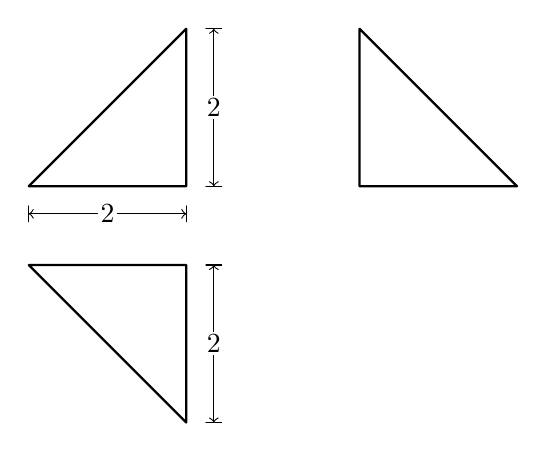
\begin{tikzpicture}[line cap=round,line join=round,scale=1]
% ---- top-left right triangle ----
\draw[thick] (0,0) -- (2,0) -- (2,2) -- cycle;

% dimensions "2" (bottom and right)
\draw[<->] (0,-0.35) -- node[fill=white,inner sep=1pt] {$2$} (2,-0.35);
\draw (0,-0.25) -- (0,-0.45);
\draw (2,-0.25) -- (2,-0.45);

\draw[<->] (2.35,0) -- node[fill=white,inner sep=1pt] {$2$} (2.35,2);
\draw (2.25,0) -- (2.45,0);
\draw (2.25,2) -- (2.45,2);

% ---- top-right right triangle (mirrored) ----
\begin{scope}[shift={(4.2,0)}]
  \draw[thick] (0,0) -- (0,2) -- (2,0) -- cycle;
\end{scope}

% ---- bottom-left right triangle (another view) ----
\begin{scope}[shift={(0,-3.0)}]
  \draw[thick] (0,2) -- (2,2) -- (2,0) -- cycle;

  \draw[<->] (2.35,0) -- node[fill=white,inner sep=1pt] {$2$} (2.35,2);
  \draw (2.25,0) -- (2.45,0);
  \draw (2.25,2) -- (2.45,2);
\end{scope}
\end{tikzpicture}
\begin{choices}
\choice{{$6 + 4\sqrt{2}$}}
\choice{{$4 + 4\sqrt{2}$}}
\choice{{$6 + 2\sqrt{3}$}}
\choice{{$4 + 2\sqrt{3}$}}
\end{choices}
\end{problem}

\begin{answer}

\end{answer}

\begin{solutions}

\end{solutions}